\documentclass{beamer}
\usepackage{../../shared/styles/custom}
\usepackage{../../shared/styles/conventions}
\usepackage{minted}

%\beamerdefaultoverlayspecification{<+->}
% \newcommand{\data}{\mathcal{D}}
% \newcommand\Item[1][]{%
% 	\ifx\relax#1\relax  \item \else \item[#1] \fi
% 	\abovedisplayskip=0pt\abovedisplayshortskip=0pt~\vspace*{-\baselineskip}}

\graphicspath{ {../assets/bias-variance/figures/} }
\setbeamertemplate{navigation symbols}{}
\newcommand{\fitpic}[1]{\begin{adjustbox}{max width=\linewidth, max totalheight=0.78\textheight}#1\end{adjustbox}}
\usetikzlibrary{arrows.meta,positioning,calc,decorations.pathreplacing}

\pgfplotsset{
  myaxis/.style={
    width=\linewidth, height=0.6\textheight,
    xmin=1, xmax=10, ymin=0.6, ymax=1.0,
    xlabel={Decision tree depth}, ylabel={Accuracy},
    ymajorgrids, grid style={gray!20, dashed},
    legend style={draw=none, fill=none, font=\small,
      /tikz/every even column/.style={column sep=8pt}},
    legend cell align=left,
    ticklabel style={font=\small},
    label style={font=\small},
  },
  trainplot/.style={very thick, blue!70!black, smooth},
  testplot/.style={very thick, red!70!black, smooth, dashed},
  regionfill/.style={draw=none, fill opacity=0.15},
}


\title{Bias-Variance and Cross Validation}
\date{\today}
\author{Nipun Batra and teaching staff}
\institute{IIT Gandhinagar}
\begin{document}
\maketitle

\begin{frame}{Table of Contents}
\tableofcontents
\end{frame}

\section{Introduction to Bias-Variance}

\begin{frame}{What is the Bias-Variance Tradeoff?}
\begin{alertbox}{The Central Challenge in Machine Learning}
\textbf{Every ML model faces a fundamental tension:}
\begin{itemize}
\item Make simple assumptions → Miss important patterns (High Bias)
\item Make complex assumptions → Overfit to noise (High Variance)
\end{itemize}
\end{alertbox}

%\vspace{0.3em}

\end{frame}

\begin{frame}{A Real-World Analogy: Weather Prediction}
\begin{examplebox}{Simple Model: "Tomorrow = Today"}
\textbf{High Bias:} Ignores weather patterns \\
\textbf{Low Variance:} Always makes same type of prediction
\end{examplebox}

\begin{examplebox}{Complex Model: 1000+ Variables}
\textbf{Low Bias:} Can capture complex patterns \\
\textbf{High Variance:} Small errors → wildly different forecasts
\end{examplebox}

\textbf{Goal:} Find the sweet spot between these extremes
\end{frame}

\begin{frame}{A Question!}
	What would be the decision boundary of a decision tree classifier? 
		
	\begin{figure}
		\centering
	\includegraphics[scale=0.55]{dataset-1}
	\end{figure}


	\end{frame}

	\begin{frame}{Decision Boundary for a tree with depth 1}
	\begin{figure}[h]
	    \centering
	    \begin{minipage}{0.45\textwidth}
	        \centering
	        \includegraphics[width=\textwidth]{example-1-depth-1-boundary}
	        \caption{Decision Boundary}
	    \end{minipage}
	    \hfill
	    \begin{minipage}{0.45\textwidth}
	        \centering
	        \includegraphics[width=\textwidth]{example-1-depth-1-decision-tree}
	        \caption{Decision Tree}
	    \end{minipage}
	\end{figure}
	\end{frame}
	
	\begin{frame}{Decision Boundary for a tree with no depth limit}
	\begin{figure}[h]
	    \centering
	    \begin{minipage}{0.45\textwidth}
	        \centering
	        \includegraphics[width=\textwidth]{example-1-nolimit-boundary}
	        \caption{Decision Boundary}
	    \end{minipage}
	    \hfill
	    \begin{minipage}{0.45\textwidth}
	        \centering
	        \includegraphics[width=\textwidth]{example-1-nolimit-decision-tree}
	        \caption{Decision Tree}
	    \end{minipage}
	\end{figure}
	\end{frame}
	

	\begin{frame}{Are deeper trees always better?}
	\only<1-2>{
	As we saw, deeper trees learn more complex decision boundaries.
	}
	
	\only<2>{
	\vspace{1cm}
	But, sometimes this can lead to poor generalization
	}	
	\end{frame}

	\begin{frame}{An example}
	Consider the dataset below
	\begin{figure}[h]
	    \centering
	    \begin{minipage}{0.45\textwidth}
	        \centering
	        \includegraphics[width=\textwidth]{dataset-2-train}
	        \caption{Train Set}
	    \end{minipage}
	    \hfill
	    \begin{minipage}{0.45\textwidth}
	        \centering
	        \includegraphics[width=\textwidth]{dataset-2-test}
	        \caption{Test Set}
	    \end{minipage}
	\end{figure}
	\end{frame}

	\begin{frame}{Underfitting}
	Underfitting is also known as high bias, since it has a very biased incorrect assumption.
	\begin{figure}[h]
	    \centering
	    \begin{minipage}{0.45\textwidth}
	        \centering
	        \includegraphics[width=\textwidth]{example-2-depth-1-boundary}
	        \caption{Decision Boundary}
	    \end{minipage}
	    \hfill
	    \begin{minipage}{0.45\textwidth}
	        \centering
	        \includegraphics[width=\textwidth]{example-2-depth-1-decision-tree}
	        \caption{Decision Tree}
	    \end{minipage}
	\end{figure}
	\end{frame}

	\begin{frame}{Overfitting}
	Overfitting is also known as high variance, since very small changes in data can lead to very different models.\\
	Decision tree learned has depth of 10.
	\begin{center}
	\includegraphics[scale=0.5]{example-2-nolimit-boundary}
	\end{center}
	\end{frame}


	\begin{frame}{Intuition for Variance}
	A small change in data can lead to very different models.\\
	\vspace{1cm}
	\begin{columns}
		\begin{column}{0.5\textwidth}{\hspace{1.75cm} Dataset 1}
			\begin{center}
			\includegraphics[width = \textwidth]{dataset-2-train}
			\end{center}
		\end{column}
		\begin{column}{0.5\textwidth}{\hspace{1.75cm} Dataset 2}
			\begin{center}
			\includegraphics[width = \textwidth]{dataset-2-train-var}
			\end{center}
		\end{column}
	\end{columns}
	\end{frame}


	\begin{frame}{Intuition for Variance}
	\begin{columns}
		\begin{column}{0.5\textwidth}
			\begin{center}
			\includegraphics[scale=0.2]{var_1}
			\end{center}
		\end{column}
		\begin{column}{0.5\textwidth}
			\begin{center}
			\includegraphics[scale=0.2]{var_2}
			\end{center}
		\end{column}
	\end{columns}
	\end{frame}


	\begin{frame}{A Good Fit}
	\begin{columns}
		\begin{column}{0.5\textwidth}
			\includegraphics[width=\textwidth]{example-2-optimal-boundary}
		\end{column}
		\begin{column}{0.5\textwidth}
			\includegraphics[width =\textwidth]{example-2-optimal-tree}
		\end{column}
	\end{columns}

	\end{frame}

	\begin{frame}{Accuracy vs Decision Tree Depth}
\centering
\begin{tikzpicture}
\begin{axis}[myaxis]
% Train
\addplot[trainplot] coordinates {
(1,0.72) (2,0.78) (3,0.83) (4,0.88) (5,0.92) (6,0.95) (7,0.97) (8,0.985) (9,0.992) (10,0.996)
}; \addlegendentry{Train accuracy}
% Test
\addplot[testplot] coordinates {
(1,0.68) (2,0.75) (3,0.81) (4,0.86) (5,0.88) (6,0.87) (7,0.84) (8,0.80) (9,0.76) (10,0.72)
}; \addlegendentry{Test accuracy}
\end{axis}
\end{tikzpicture}
\end{frame}


% ============================================================
% 2) Underfitting (High Bias)
% ============================================================
\begin{frame}{Underfitting (High Bias) Region}
\centering
\begin{tikzpicture}
\begin{axis}[myaxis]
% Shaded region (left) — not in legend
\addplot[regionfill, fill=blue!50, forget plot]
  coordinates {(1,0.6) (2.6,0.6) (2.6,1.0) (1,1.0)} -- cycle;

% Curves (these appear in legend as lines)
\addplot[trainplot] coordinates {
(1,0.72) (2,0.78) (3,0.83) (4,0.88) (5,0.92) (6,0.95) (7,0.97) (8,0.985) (9,0.992) (10,0.996)
}; \addlegendentry{Train}
\addplot[testplot] coordinates {
(1,0.68) (2,0.75) (3,0.81) (4,0.86) (5,0.88) (6,0.87) (7,0.84) (8,0.80) (9,0.76) (10,0.72)
}; \addlegendentry{Test}

% Manual legend swatch for the region (rectangle)
\addlegendimage{area legend, draw=blue!60!black, fill=blue!50, fill opacity=0.15}
\addlegendentry{Underfitting / High Bias}
\end{axis}
\end{tikzpicture}
\end{frame}

% ============================================================
% 3) Overfitting (High Variance)
% ============================================================
\begin{frame}{Overfitting (High Variance) Region}
\centering
\begin{tikzpicture}
\begin{axis}[myaxis]
% Shaded region (right) — not in legend
\addplot[regionfill, fill=red!60, forget plot]
  coordinates {(7.6,0.6) (10,0.6) (10,1.0) (7.6,1.0)} -- cycle;

% Curves
\addplot[trainplot] coordinates {
(1,0.72) (2,0.78) (3,0.83) (4,0.88) (5,0.92) (6,0.95) (7,0.97) (8,0.985) (9,0.992) (10,0.996)
}; \addlegendentry{Train}
\addplot[testplot] coordinates {
(1,0.68) (2,0.75) (3,0.81) (4,0.86) (5,0.88) (6,0.87) (7,0.84) (8,0.80) (9,0.76) (10,0.72)
}; \addlegendentry{Test}

% Manual legend swatch for the region (rectangle)
\addlegendimage{area legend, draw=red!70!black, fill=red!60, fill opacity=0.15}
\addlegendentry{Overfitting / High Variance}
\end{axis}
\end{tikzpicture}
\end{frame}


% ============================================================
% 4) Good Fit (Sweet Spot)
% ============================================================
\begin{frame}{Good Fit (Sweet Spot) Region}
\centering
\begin{tikzpicture}
\begin{axis}[myaxis]
% Shaded region (middle) — not in legend
\addplot[regionfill, fill=green!60!black, forget plot]
  coordinates {(3,0.6) (7,0.6) (7,1.0) (3,1.0)} -- cycle;

% Mark an "optimal" depth near the test peak (kept within bounds)
\addplot[only marks, mark=star*, mark options={scale=1.2}] coordinates {(5.5,0.87)};
\node[font=\scriptsize, anchor=north] at (axis cs:5.5,0.865) {optimal};

% Curves
\addplot[trainplot] coordinates {
(1,0.72) (2,0.78) (3,0.83) (4,0.88) (5,0.92) (6,0.95) (7,0.97) (8,0.985) (9,0.992) (10,0.996)
}; \addlegendentry{Train}
\addplot[testplot] coordinates {
(1,0.68) (2,0.75) (3,0.81) (4,0.86) (5,0.88) (6,0.87) (7,0.84) (8,0.80) (9,0.76) (10,0.72)
}; \addlegendentry{Test}

% Manual legend swatch for the region (rectangle)
\addlegendimage{area legend, draw=green!70!black, fill=green!60!black, fill opacity=0.15}
\addlegendentry{Good Fit / Balance Bias \& Variance}
\end{axis}
\end{tikzpicture}
\end{frame}


	\begin{frame}{The Fundamental Question: Model Complexity}
\begin{alertbox}{What We Just Observed}
	\scriptsize
\begin{itemize}
\item \textbf{Depth 1}: Simple boundary, might miss patterns (underfitting)
\item \textbf{No depth limit}: Complex boundary, might memorize noise (overfitting)
\end{itemize}
\end{alertbox}

\begin{keypointsbox}
\textbf{This Leads to Three Key Concepts:}
\scriptsize
\begin{enumerate}
\item \textbf{Bias}: How much do our assumptions limit our model's ability to learn?
\item \textbf{Variance}: How much does our model change with different training data?
\item \textbf{Irreducible Error}: The noise we can never eliminate
\end{enumerate}
\end{keypointsbox}

\textbf{The Bias-Variance Tradeoff}: We can't minimize both bias and variance simultaneously!
\end{frame}

\begin{frame}{Dartboard Analogy: Four Scenarios}
\fitpic{
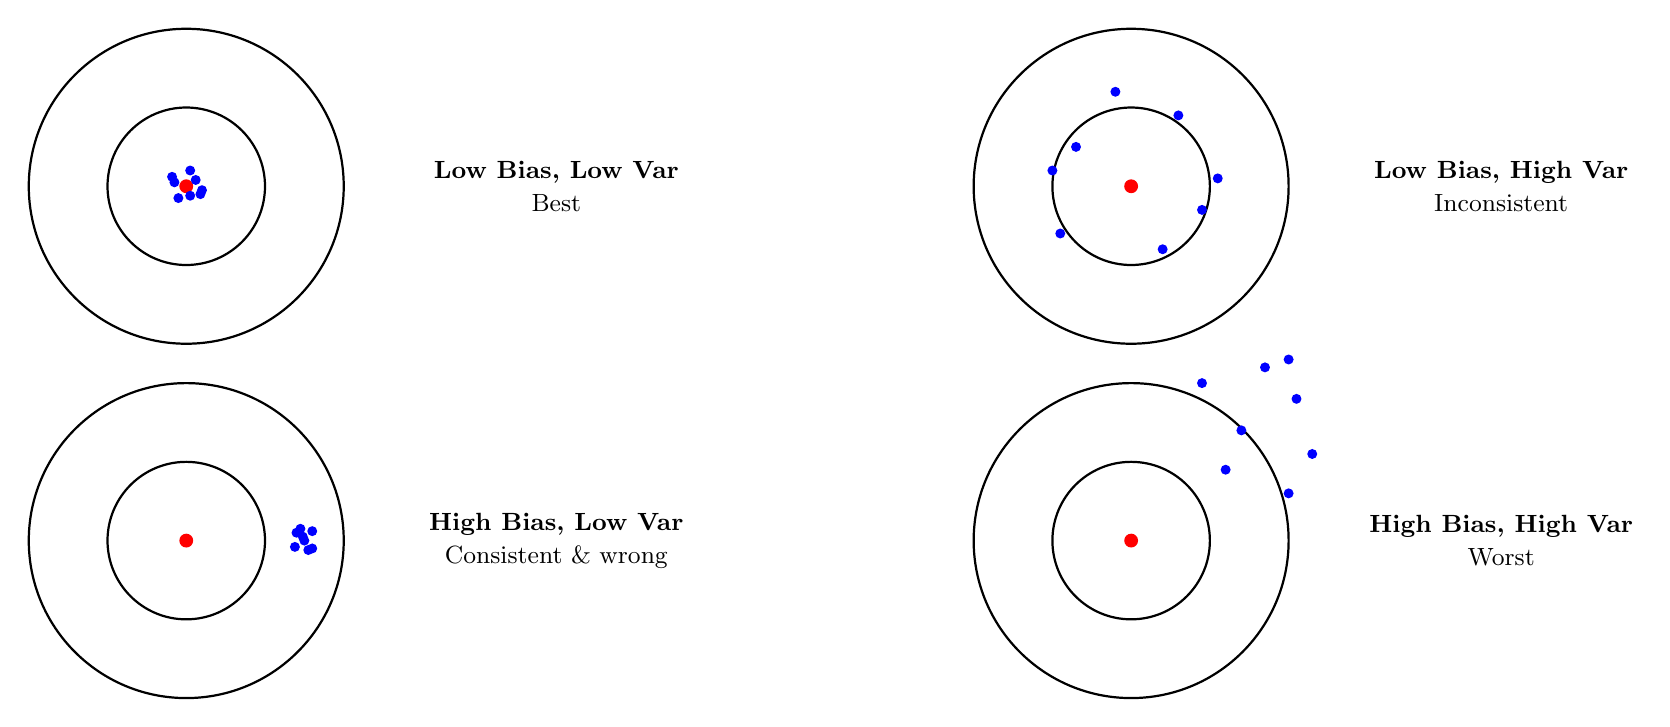
\begin{tikzpicture}
  % --- helper: draw one target with a given point list ---
  \tikzset{dotp/.style={circle, fill=blue, minimum size=1.8pt, inner sep=0pt}}

  % Low Bias, Low Variance (tight near center)
  \begin{scope}[shift={(-6,2)}]
    \draw[thick] (0,0) circle (2.0);
    \draw[thick] (0,0) circle (1.0);
    \fill[red] (0,0) circle (2.5pt);
    \def\Points{(0.12,0.08),(0.18,-0.10),(-0.15,0.05),(0.05,0.20),(-0.10,-0.15),(0.20,-0.05),(-0.18,0.12),(0.05,-0.12)}
    \foreach \P in \Points { \fill[blue] \P circle (1.8pt); }
    \node[align=center] at (4.7,0) {\small \textbf{Low Bias, Low Var}\\\small Best};
  \end{scope}

  % Low Bias, High Variance (scattered around center)
  \begin{scope}[shift={(6,2)}]
    \draw[thick] (0,0) circle (2.0);
    \draw[thick] (0,0) circle (1.0);
    \fill[red] (0,0) circle (2.5pt);
    \def\Points{(0.6,0.9),(-0.7,0.5),(0.4,-0.8),(-0.9,-0.6),(1.1,0.1),(-0.2,1.2),(0.9,-0.3),(-1.0,0.2)}
    \foreach \P in \Points { \fill[blue] \P circle (1.8pt); }
    \node[align=center] at (4.7,0) {\small \textbf{Low Bias, High Var}\\\small Inconsistent};
  \end{scope}

  % High Bias, Low Variance (tight off-center)
  \begin{scope}[shift={(-6,-2.5)}]
    \draw[thick] (0,0) circle (2.0);
    \draw[thick] (0,0) circle (1.0);
    \fill[red] (0,0) circle (2.5pt);
    \def\Points{(1.5,0.0),(1.4,0.1),(1.6,-0.1),(1.45,0.15),(1.55,-0.12),(1.48,0.05),(1.6,0.12),(1.38,-0.08)}
    \foreach \P in \Points { \fill[blue] \P circle (1.8pt); }
    \node[align=center] at (4.7,-0) {\small \textbf{High Bias, Low Var}\\\small Consistent \& wrong};
  \end{scope}

  % High Bias, High Variance (scattered off-center)
  \begin{scope}[shift={(6,-2.5)}]
    \draw[thick] (0,0) circle (2.0);
    \draw[thick] (0,0) circle (1.0);
    \fill[red] (0,0) circle (2.5pt);
    \def\Points{(1.4,1.4),(2.0,0.6),(0.9,2.0),(2.1,1.8),(1.7,2.2),(2.3,1.1),(1.2,0.9),(2.0,2.3)}
    \foreach \P in \Points { \fill[blue] \P circle (1.8pt); }
    \node[align=center] at (4.7,-0) {\small \textbf{High Bias, High Var}\\\small Worst};
  \end{scope}
\end{tikzpicture}
}
\end{frame}


\begin{frame}{Mathematical Foundation: Bias-Variance Decomposition}
\begin{definitionbox}{The Fundamental Equation}
For any learning algorithm, the expected prediction error can be decomposed as:
$$\text{Expected Error} = \text{Bias}^2 + \text{Variance} + \text{Irreducible Error}$$
\end{definitionbox}

Where:
\begin{itemize}
\item $\text{Bias}^2 = (\mathbb{E}[\hat{f}(x)] - f(x))^2$ \\
  \textit{Squared difference between average prediction and true function}
\item $\text{Variance} = \mathbb{E}[(\hat{f}(x) - \mathbb{E}[\hat{f}(x)])^2]$ \\
  \textit{Expected squared deviation from average prediction}
\item $\text{Irreducible Error} = \sigma^2$ \\
  \textit{Noise in the data that no model can eliminate}
\end{itemize}
\end{frame}

\begin{frame}{Intuitive Understanding of Each Component}
\begin{examplebox}{Bias: "Are we systematically wrong?"}
	\scriptsize
\begin{itemize}
\item High Bias: Linear model fitting curved data
\item Low Bias: Flexible model that can approximate true function
\item \textbf{Think}: Average error if we could train on infinite datasets
\end{itemize}
\end{examplebox}

\begin{examplebox}{Variance: "Are we consistently wrong?"}
	\scriptsize
\begin{itemize}
\item High Variance: Model predictions change drastically with new training data
\item Low Variance: Model predictions remain stable across different datasets
\item \textbf{Think}: How much do predictions fluctuate between training runs?
\end{itemize}
\end{examplebox}

\textbf{Key Insight:} Both contribute to total error, but reducing one often increases the other!
\end{frame}

	% \begin{frame}{Accuracy vs Depth Curve}
	% 	\begin{center}
	% 	\includegraphics[scale=0.55]{acc-depth-plot}
	% \end{center}
	% \pause As depth increases, train accuracy improves\\
	% \pause As depth increases, test accuracy improves till a point\\
	% \pause At very high depths, test accuracy is not good (overfitting). 

	% \end{frame}

	% \begin{frame}{Accuracy vs Depth Curve : Underfitting}
	% The highlighted region is the underfitting region.\\
	% Model is too simple (less depth) to learn from the data. 
	% \begin{center}
	% \includegraphics[scale=0.55]{acc-depth-plot-underfit}
	% \end{center}
	% \end{frame}

	% \begin{frame}{Accuracy vs Depth Curve : Overfitting}
	% The highlighted region is the overfitting region.\\
	% Model is complex (high depth) and hence also learns the anomalies in data. 
	% \begin{center}
	% \includegraphics[scale=0.55]{acc-depth-plot-overfit}
	% \end{center}
	% \end{frame}

	% \begin{frame}{Accuracy vs Depth Curve }
	% The highlighted region is the good fit region.\\
	% We want to maximize test accuracy while being in this region.
	% \begin{center}
	% \includegraphics[scale=0.55]{acc-depth-plot-properfit}
	% \end{center}
	% \end{frame}

	\begin{frame}{The big question!?}
	\only<1-2>{
	How to find the optimal depth for a decision tree?\\
	}
	\only<2>{
	\vspace{1cm}
	Use cross-validation!
	}
	\end{frame}


	\begin{frame}{Our General Training Flow}
	\includegraphics[width = \textwidth]{../assets/bias-variance/diagrams/general-workflow}
	\end{frame}

	\begin{frame}[fragile]{Example: Training and Evaluation}
\textbf{Step-by-step:}



\begin{block}{Python Example: Decision Tree with fixed depth}
\scriptsize
\begin{verbatim}
# 1. Load dataset
X, y = load_iris(return_X_y=True)
X_train, X_test, y_train, y_test = train_test_split(
    X, y, test_size=0.3, random_state=42)
# 2. Train model with fixed hyperparameter
clf = DecisionTreeClassifier(max_depth=3, random_state=42)
clf.fit(X_train, y_train)
# 3. Evaluate
train_acc = accuracy_score(y_train, clf.predict(X_train))
test_acc = accuracy_score(y_test, clf.predict(X_test))
print(f"Max Depth: 3 | Train Acc: {train_acc:.2f} | Test Acc: {test_acc:.2f}")
\end{verbatim}
\end{block}

\textbf{Sample Output:}
\begin{itemize}
    \item Max Depth: 3
    \item Train Accuracy: 0.98
    \item Test Accuracy: 0.96
\end{itemize}
\end{frame}


\begin{frame}{Single Train-Test Split: Setup}
\textbf{Scenario:}  
We trained with \texttt{max\_depth=3} and got good test accuracy.

\pause
\begin{block}{Our Current Setup}
\begin{itemize}
    \item One fixed train/test split
    \item Train on training set, evaluate on test set
    \item Hyperparameter: \texttt{max\_depth=3} (chosen arbitrarily)
\end{itemize}
\end{block}

\pause
\begin{block}{Example Results}
\small
\begin{tabular}{lcc}
\toprule
Max Depth & Train Acc & Test Acc \\
\midrule
2 & 0.95 & 0.94 \\
3 & 0.98 & 0.96 \\
4 & 1.00 & 0.92 \\
\bottomrule
\end{tabular}
\end{block}
\end{frame}

\begin{frame}{Limitations of a Single Train-Test Split}
\begin{block}{Why This Can Be Misleading}
		\scriptsize

\begin{itemize}
    \item Test accuracy depends on how the split was made
    \item A lucky/unlucky split can overestimate or underestimate performance
    \item We might miss the \textbf{true best hyperparameter}
\end{itemize}
\end{block}

\pause
\begin{alertblock}{Key Insight}
		\scriptsize

Even though \texttt{max\_depth=3} looks best here,  
it might not be the best for another random split.
\end{alertblock}

\pause
\begin{block}{What We Need}
	\scriptsize
\begin{itemize}
    \item Evaluate using \textbf{all} data for testing
    \item Avoid overfitting to a single test set
\end{itemize}
\end{block}

\end{frame}


	\begin{frame}{K-Fold cross-validation: Utilise full dataset for testing}
	\includegraphics[width = \textwidth]{../assets/bias-variance/diagrams/cross-validation-train-test.pdf}
	\end{frame}

\begin{frame}[fragile]{Example: K-Fold Cross-Validation (Fixed Depth)}
\textbf{Step-by-step:}

\begin{block}{Python Example: Decision Tree with fixed depth, using 5-Fold CV}
\scriptsize
\begin{verbatim}
kf = KFold(n_splits=5, shuffle=True, random_state=42)
acc_scores = []

for train_idx, test_idx in kf.split(X):
    X_train, X_test = X[train_idx], X[test_idx]
    y_train, y_test = y[train_idx], y[test_idx]
    
    clf = DecisionTreeClassifier(max_depth=3, random_state=42)
    clf.fit(X_train, y_train)
    
    acc_scores.append(accuracy_score(y_test, clf.predict(X_test)))

print(f"Max Depth: 3 | Mean Test Acc: {np.mean(acc_scores):.2f}")
\end{verbatim}
\end{block}

\textbf{Sample Output:}
\begin{itemize}
    \item \texttt{Max Depth: 3 | Mean Test Acc: 0.95}
\end{itemize}
\end{frame}

\begin{frame}{K-Fold Cross-Validation: Insights \& Next Steps}
\textbf{What improves here?}
\begin{itemize}
    \item We now test performance on \textbf{multiple test sets} (one per fold).
    \item This gives a \textbf{more reliable estimate} of generalization accuracy.
\end{itemize}

\pause
\textbf{But... what is the \emph{final model}?}
\begin{itemize}
    \item In K-Fold CV, the model is re-trained for each fold — no single final model exists yet.
    \item After estimating performance, we can:
    \begin{itemize}
        \item Re-train on the \textbf{entire dataset} with the chosen hyperparameters.
        \item Deploy this re-trained model.
    \end{itemize}
\end{itemize}
\end{frame}

	\begin{frame}{The Validation Set}
	\includegraphics[width = \textwidth]{../assets/bias-variance/diagrams/validation-workflow}
	\end{frame}

	\begin{frame}[fragile]{Train/Validation/Test: Hyperparameter Tuning}
\textbf{Idea:} Split training set into smaller \textbf{train} and \textbf{validation} parts.

\begin{block}{Python Example: Loop over depths}
\tiny
\begin{verbatim}
# Split: Train+Val and Test
X_temp, X_test, y_temp, y_test = train_test_split(X, y,
                                                  test_size=0.3,
                                                  random_state=42)
# Split: Train and Val
X_train, X_val, y_train, y_val = train_test_split(X_temp, y_temp,
                                                  test_size=0.2,
                                                  random_state=42)

best_depth, best_val_acc = None, 0
for depth in [2, 3, 4, 5, 6]:
    clf = DecisionTreeClassifier(max_depth=depth, random_state=42)
    clf.fit(X_train, y_train)
    val_acc = accuracy_score(y_val, clf.predict(X_val))
    if val_acc > best_val_acc:
        best_val_acc, best_depth = val_acc, depth

# Retrain on Train+Val with best depth
final_clf = DecisionTreeClassifier(max_depth=best_depth, random_state=42)
final_clf.fit(X_temp, y_temp)

test_acc = accuracy_score(y_test, final_clf.predict(X_test))
print(f"Best depth: {best_depth}, Test Acc: {test_acc:.2f}")
\end{verbatim}
\end{block}
\end{frame}

\begin{frame}{Why Use a Validation Set?}
\textbf{Key Advantages:}
\begin{itemize}
    \item Allows testing \textbf{multiple hyperparameters} (e.g., decision tree depth)
    \item Prevents \textbf{overfitting to the test set}
    \item Gives a clear \textbf{criterion for choosing the best model}
    \item Final test accuracy is now a \textbf{realistic estimate of generalization}
\end{itemize}

\pause
\textbf{Limitations:}
\begin{itemize}
    \item Validation set is \textbf{only one split} of the data
    \item May not represent all possible variations in the data
\end{itemize}

\pause
\textbf{Next:} How to make use of \textbf{all possible validation splits} $\rightarrow$ \textbf{Nested Cross-Validation}.
\end{frame}



	\begin{frame}{Nested Cross Validation}
	Divide your training set into $k$ equal parts.\\
	 Cyclically use 1 part as ``validation set'' and the rest for training.\\
	Here $k = 4$
	\begin{center}
	\includegraphics[scale=0.7]{../assets/bias-variance/diagrams/cross-validation}
	\end{center}
	\end{frame}

	\begin{frame}{Nested Cross Validation}
	Average out the validation accuracy across all the folds\\
	Use the model with highest validation accuracy\\
	\includegraphics[width = \textwidth]{../assets/bias-variance/diagrams/cross-validation-avg}
	\end{frame}


	\begin{frame}[fragile]{Nested CV (Inner tuning, Outer testing)}
\tiny
\begin{verbatim}
outer_kf = KFold(n_splits=5, shuffle=True, random_state=42)
depths = [2, 3, 4, 5, 6]
outer_scores, chosen_depths = [], []

for ot_tr, ot_te in outer_kf.split(X):
    X_tr, X_te = X[ot_tr], X[ot_te]
    y_tr, y_te = y[ot_tr], y[ot_te]
    best_d, best_cv = None, -1

    # Inner CV to pick best depth
    for d in depths:
        scores = []
        for in_tr, in_val in KFold(3, shuffle=True, random_state=42).split(X_tr):
            clf = DecisionTreeClassifier(max_depth=d, random_state=42)
            clf.fit(X_tr[in_tr], y_tr[in_tr])
            scores.append(accuracy_score(y_tr[in_val],
                                         clf.predict(X_tr[in_val])))
        if np.mean(scores) > best_cv:
            best_cv, best_d = np.mean(scores), d

    chosen_depths.append(best_d)
    clf = DecisionTreeClassifier(max_depth=best_d, random_state=42)
    clf.fit(X_tr, y_tr)
    outer_scores.append(accuracy_score(y_te, clf.predict(X_te)))

print(np.mean(outer_scores), chosen_depths)
\end{verbatim}
\end{frame}

\begin{frame}{Nested CV: What You Get}
\textbf{Per outer fold:}
\begin{itemize}
  \item A \emph{chosen hyperparameter} (from inner CV)
  \item An \emph{unbiased test score} (on the outer test split)
\end{itemize}

\textbf{Overall:}
\begin{itemize}
  \item Report \(\text{mean} \pm \text{std}\) of outer test accuracy
  \item \emph{Final model}: retrain on \(\text{all data}\) with a chosen hyperparameter (e.g., the most frequent/best-average depth from inner CV)
\end{itemize}
\end{frame}



% Preamble (once):
% \usepackage{booktabs}
% \usepackage[table]{xcolor}

\begin{frame}{Nested CV: Inner-CV Matrix \& Outer Scores}
\centering
\scriptsize
\renewcommand{\arraystretch}{1.2}
\newcommand{\bestcell}{\cellcolor{green!20}\bfseries}

\resizebox{\linewidth}{!}{
\begin{tabular}{c
                S[table-format=1.3] S[table-format=1.3] S[table-format=1.3] S[table-format=1.3] S[table-format=1.3]
                c c}
\toprule
& \multicolumn{5}{c}{\textbf{Inner CV mean accuracy (by depth)}} & & \\
\cmidrule(lr){2-6}
\textbf{Outer fold} &
\texttt{d=2} & \texttt{d=3} & \texttt{d=4} & \texttt{d=5} & \texttt{d=6} &
\textbf{Chosen $d$} &
\textbf{Outer test acc} \\
\midrule
1 & 0.940 & \bestcell 0.960 & 0.950 & 0.930 & 0.900 & 3 & 0.95 \\
2 & 0.950 & \bestcell 0.965 & 0.940 & 0.920 & 0.900 & 3 & 0.96 \\
3 & 0.910 & 0.920 & \bestcell 0.935 & 0.930 & 0.910 & 4 & 0.93 \\
4 & 0.940 & \bestcell 0.955 & 0.940 & 0.930 & 0.900 & 3 & 0.95 \\
5 & \bestcell 0.945 & 0.940 & 0.935 & 0.920 & 0.900 & 2 & 0.94 \\
\midrule
\textbf{Mean across folds} &
0.937 & \bestcell 0.948 & 0.940 & 0.926 & 0.902 & & \textbf{0.95 $\pm$ 0.01} \\
\bottomrule
\end{tabular}
}

\vspace{0.5em}
\footnotesize
\textit{Interpretation:} Best inner-CV per fold is highlighted; overall best hyperparameter by inner-CV mean is \(\texttt{max\_depth}=3\).
For reporting performance, use the \emph{outer} scores: \(\mathbf{0.95 \pm 0.01}\).
\end{frame}





\begin{frame}{Next time: Ensemble Learning}
\begin{itemize}
	\item How to combine various models?
	\item Why to combine multiple models?
	\item How can we reduce bias?
	\item How can we reduce variance?
\end{itemize}
\end{frame}




\end{document}
